\documentclass[11pt, oneside]{article}   	% use "amsart" instead of "article" for AMSLaTeX format
\usepackage{geometry}                		% See geometry.pdf to learn the layout options. There are lots.
\geometry{letterpaper}                   		% ... or a4paper or a5paper or ... 
%\geometry{landscape}                		% Activate for rotated page geometry
%\usepackage[parfill]{parskip}    		% Activate to begin paragraphs with an empty line rather than an indent
\usepackage{graphicx}				% Use pdf, png, jpg, or eps§ with pdflatex; use eps in DVI mode
								% TeX will automatically convert eps --> pdf in pdflatex		
\usepackage{amssymb}
\usepackage{minted}


%SetFonts

%SetFonts


\title{Brief Article}
\author{The Author}
%\date{}							% Activate to display a given date or no date

\begin{document}
\begin{flushright}
Donovan Guelde\\
CSCI 5352\\
PS4\\
\end{flushright}
1.  a.  Given: $\epsilon = c_{in}-c_{out},\ 2c = c_{in} + c_{out},\ p_{out}=\frac{c_{out}}{n},\ p_{in}=\frac{c_{in}}{n}$\\
\indent\indent $c_{in} = \epsilon + c_{out} = 2c-c_{out}$\\
\indent\indent $c_{out} = \frac{2c-\epsilon}{2}$\\
\indent\indent $c_{out} = c_{in}-\epsilon= 2c-c_{in}$\\
\indent\indent $c_{in} = \frac{2c+\epsilon}{2}$\\
\indent\indent $p_{in} = \frac{2c+\epsilon}{2n},$ and  $p_{out} = \frac{2c-\epsilon}{2n}$\\\\\\
1.  b.  To study the simple SI model as discussed in class, the networkx library function planted\_partition\_graph() was used to generate planted partition networks, where $p_{in}$ and $p_{out}$ were derived from $\epsilon$.  To determine average length and size of epidemics, $\epsilon$\\ was fixed at 0, and p was raised from 0.0 to 1.0 in increments of 0.01.  For each value of p, 200 graphs were generated via the planted\_partition\_graph() function, and 200 epidemic simulations were performed on each graph.  This resulted in relatively smooth plots for average length and average size.\\
\indent Plotting average epidemic size as a function of p gives the following results:\\
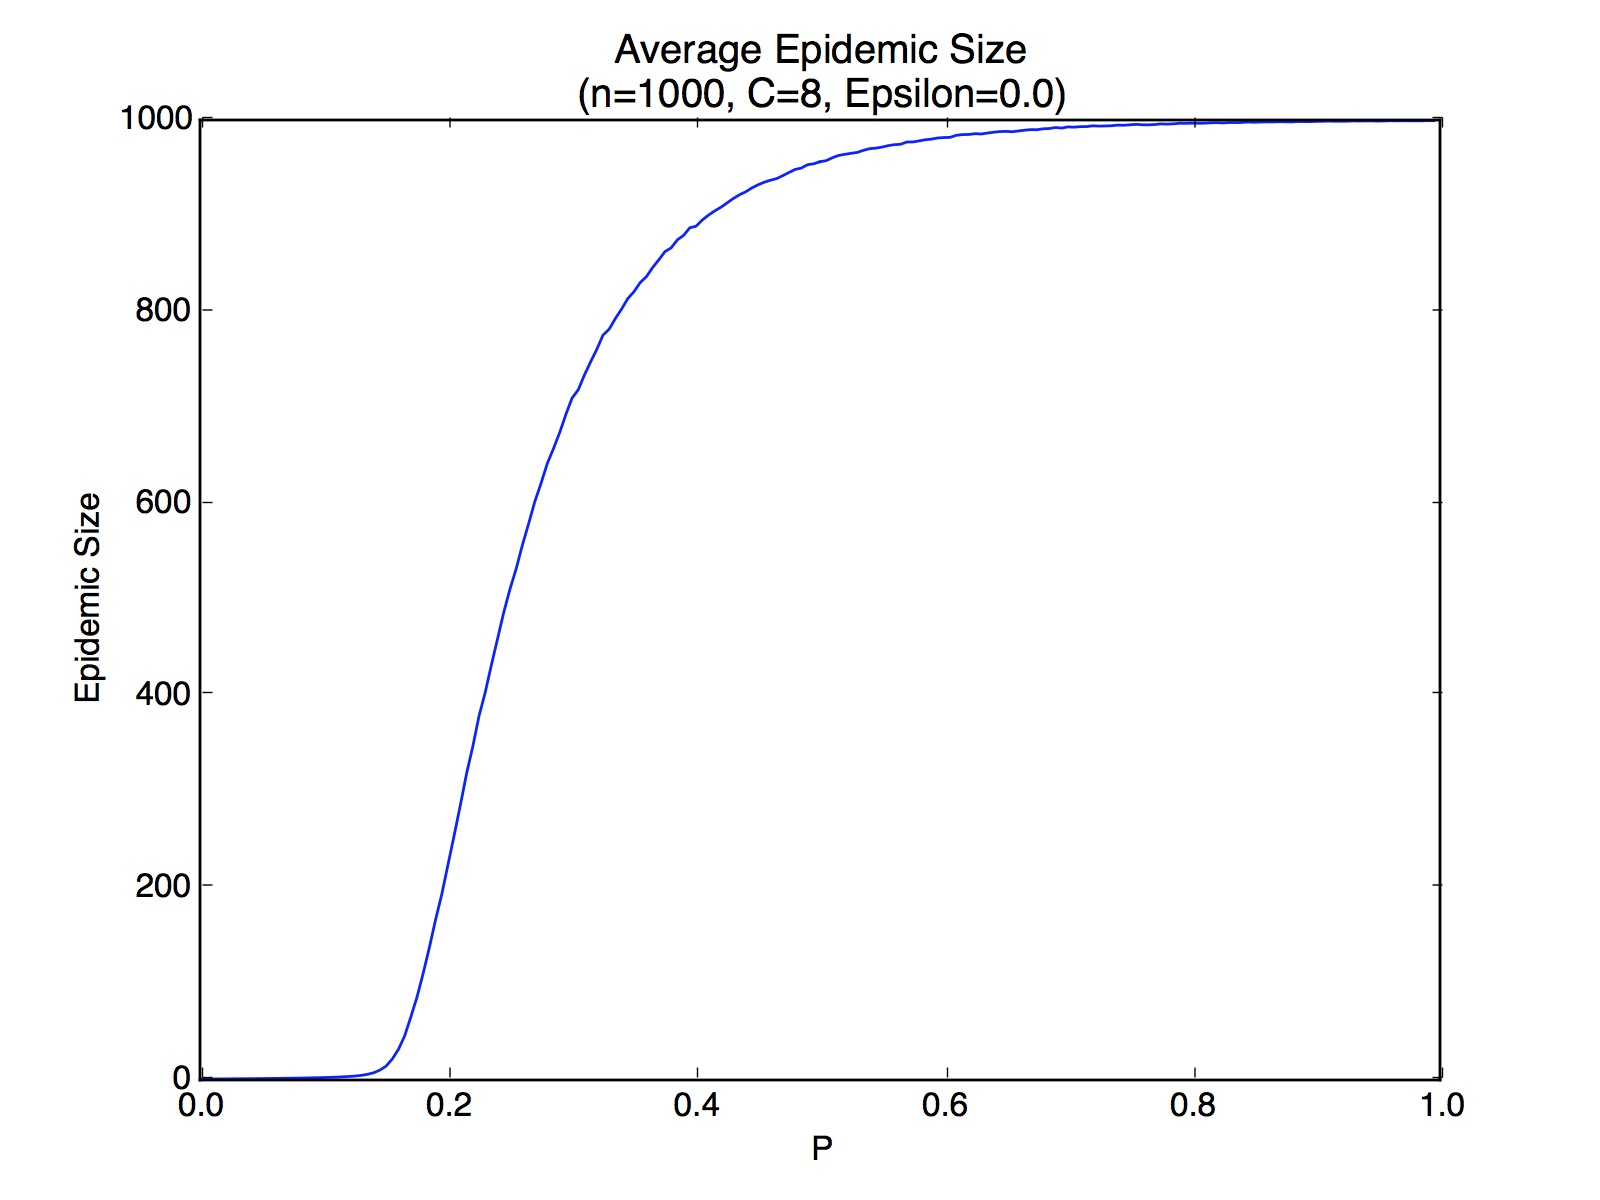
\includegraphics[scale=0.23]{size}\\
\indent The epidemic size plot shows three distinct regions.  First, there is a nearly flat area where epidemic size is very close to 1.  This correlates to low p values, from 0.0 to approximately 0.17.  This is expected, as at p=0.0, it is impossible for the epidemic to spread past the 'patient zero' node.  As p increases up to 0.17, the low probability of infection makes the spread of the epidemic very unlikely past a few additional nodes past patient zero.  As each node has mean degree 8, the expected number of infections caused by patient zero is $8p = 1.36$ at p = 0.17.  The infection will spread by just a few nodes at such low p values.  As p increases past 0.18, a pattern analogous to the random graph phase change can be seen.  As the number of expected infections per contagious node grows larger, the epidemic size increases very rapidly.  In this region of the plot, each infected node infects, on average, more than one neighboring nodes (ignoring nodes already infected).  Due to the specified value of $\epsilon$, the number of a node's edges that are internal to its group is, on average, the same as the number of edges connecting it to the other group.  This allows the infection to spread easily between the groups, and makes it possible for the infection to reach all nodes without structural hinderance.\\
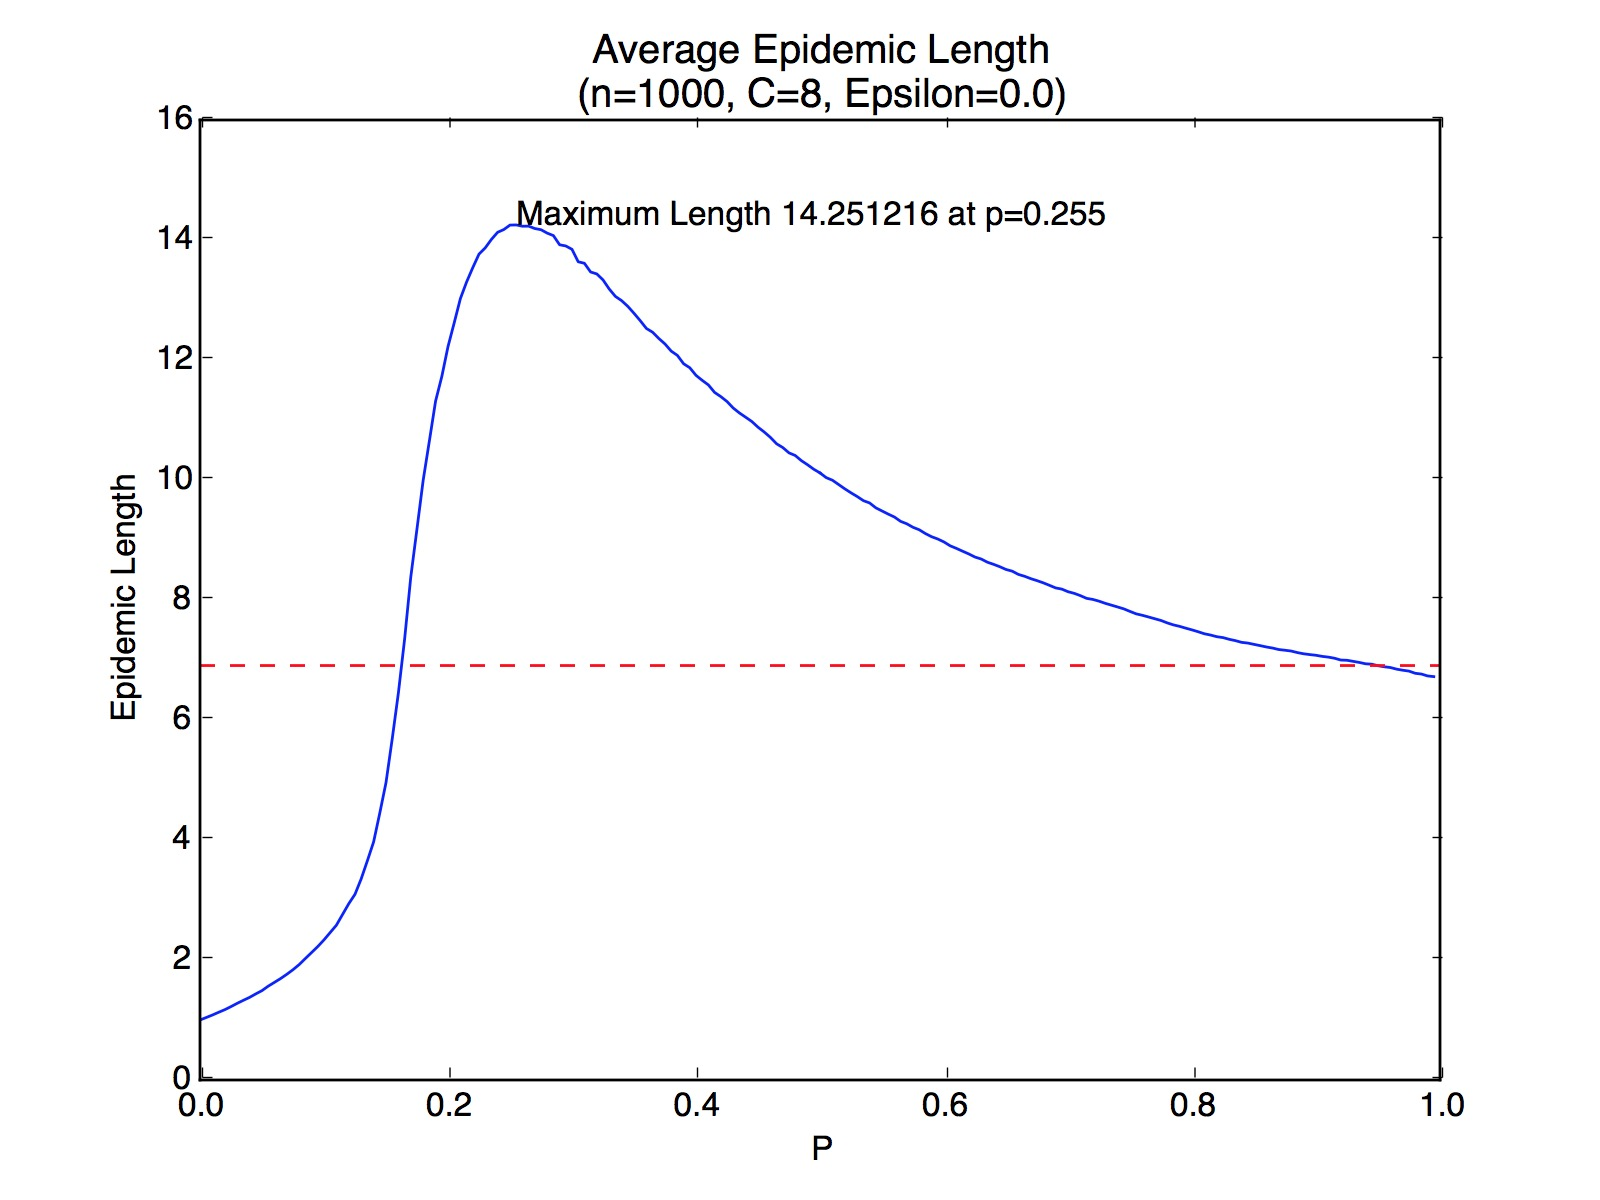
\includegraphics[scale=0.23]{length}\\
\indent Epidemic length also grows slowly at low p values, a reflection of the low epidemic size.  Since we have set up the epidemic simulation in such a way that a node is only contagious for a single time $t$, there is no opportunity to infect other nodes at time $t+1$ and beyond.  This limited window of infection, combined with a low probability of infection, means that patient zero may occasionally infect a neighbor node, which, with low probability, may infect a neighbor in turn.  In other words, at low probability of infection, the epidemic quickly dies out.  Average epidemic length does not surpass 2 until p =  0.17, where average size was found to be 2.02.  Once p reaches the critical point seen in the size plot, epidemic length quickly increases.  When the number of expected infections caused by each newly infected node is low, but approaches 2, epidemic length increases dramatically.  Interestingly, p=0.255 gives the maximum epidemic length, while this corresponds to a relatively low epidemic size of approximately 400.  At this p value, the expected number of new infections per node infected at time (t-1) is 7p = 1.785 (8 edges - 1 edge for incoming infection, ignoring the possibility that another neighbor is already infected).  This means that the epidemic is spreading in a mostly linear, rather than tree-like, fashion, allowing length to increase while size is still well below n.  As p grows and each infected node is expected to produce more infections among its neighbors, the length decreases, approaching log(n), reflecting a branching epidemic spread.  As p approaches 1, nearly every neighbor of an infected node will become infected itself, and the epidemic length approaches the diameter of the graph.\\\\\\
1. c.  To examine how the behavior of the epidemic is affected by the large-scale structure of the network, planted\_partition\_graph() was used to create planned partition graphs, and these graphs were used in simulations for $\epsilon$ values of 0 to 16, in steps of 0.1, and p values of 0 to 1, in steps of 0.01.  100 graphs were generated for each $\epsilon$/p value pair, and 100 simulations ere conducted per graph.  Plotting $\epsilon$,p, and epidemic length as a surface plot gives very clear indication of the effect of community structure on epidemic behavior.  There is a high peak in length when $\epsilon$ is between 15 and 16, and p is approximately 0.3.  Focussing specifically in this area, maximum epidemic length was found at p=.32, as $\epsilon$ approaches 16.\\
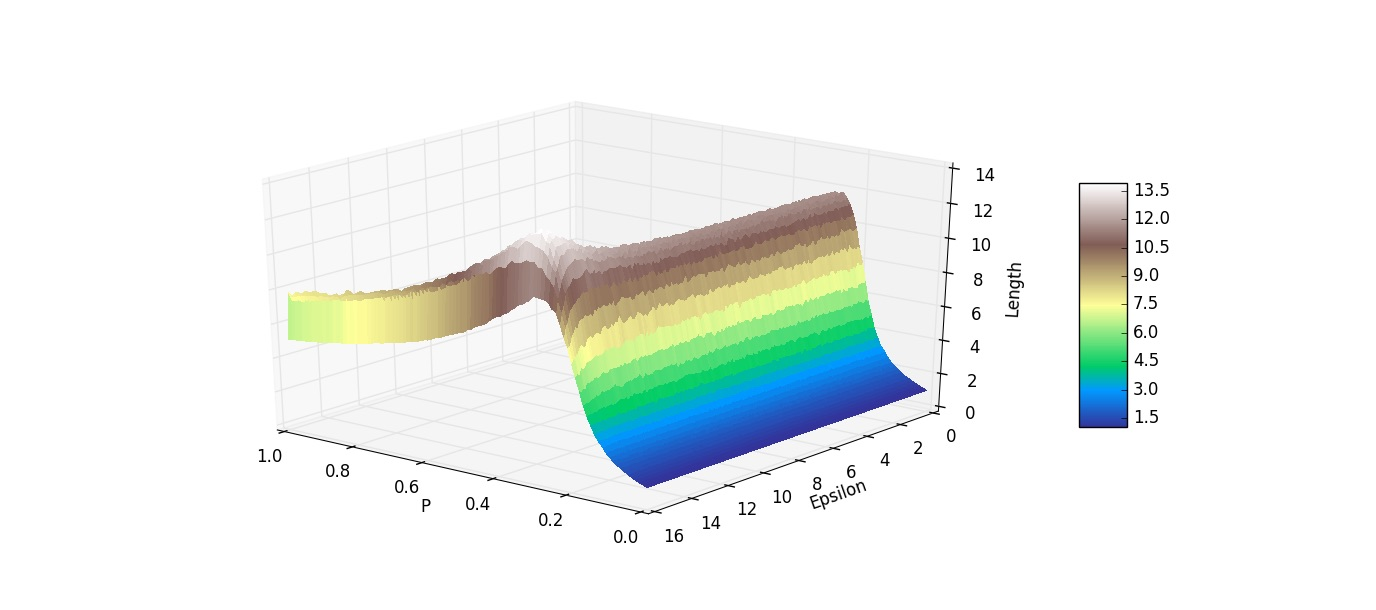
\includegraphics[scale=0.33]{last.jpg}\\
\indent Holding p fixed at 0.32, and varying $\epsilon$ from 0 to 16 gives the following results for epidemic length:\\
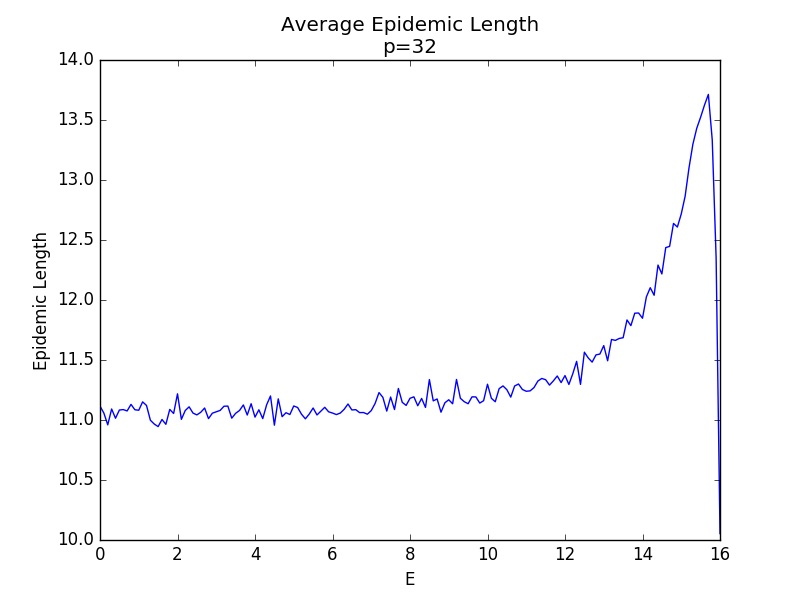
\includegraphics[scale=0.5]{P32length}\\
\indent At such high $\epsilon$ values, there are few edges connecting the two groups.  As $\epsilon$ gets larger, edges between groups decreases.  With just a few connecting edges, yet a high p value, the group where the epidemic did not originate acts to extend the effective network diameter, as far as the epidemic is concerned.  Rather than a diameter of log(n), the epidemic experiences a diameter of 2 log (n/2).  The effect of this diameter extension would vary randomly depending on what time t the epidemic spread reaches one of the few edges connecting the groups.\\
\includegraphics[scale=0.5]{p32size}\\
\indent For this same p value, epidemic size shows a steep drop after the maximum point observed in the length graph above.  This is caused by the separation of the two groups as $p_{in}$ nears 0.0.  With no way to reach the $\frac{n}{2}$ nodes in the other component, epidemic size is limited to $\frac{n}{2}$.  The relatively low p value of .32 acts to keep maximum infection size below this level, however.\\\\\\\\\\\\\\\\\\\\\\\\\\\\\\\\\\\\
\inputminted[linenos,fontsize=\scriptsize]{python}{fastq1.py}
\end{document}  